%! Author = Omar Iskandarani
%! Title = ...
%! Date = xx-xx-2025
%! Affiliation = Independent Researcher, Groningen, The Netherlands
%! License = © 2025 Omar Iskandarani. All rights reserved. This manuscript is made available for academic reading and citation only. No republication, redistribution, or derivative works are permitted without explicit written permission from the author. Contact: info@omariskandarani.com
%! ORCID = 0009-0006-1686-3961
%! DOI = 10.5281/zenodo.xxxxxxx

% === Metadata ===
\newcommand{\papertitle}{Photon as a Topological Vortex Ring: \\ Torsion and the Geometry of Light in the Æther}
\newcommand{\paperdoi}{10.5281/zenodo.xxxxxxxx}

\documentclass[twocolumn,aps,pre,floatfix,nofootinbib]{revtex4-2}
\usepackage{amsmath, amssymb}
\usepackage{graphicx}
\usepackage{float}
\usepackage{booktabs}
\usepackage{xcolor}
\usepackage{tcolorbox}
\usepackage{hyperref}
\usepackage{enumitem}
\usepackage{physics}
\usepackage{caption}
\usepackage{bm}
\usepackage{tikz}
\usepackage{pgfplots}
\usepackage{lmodern}
\usepackage{amsmath,amssymb,amsfonts}
\usepackage{mathtools}
\usetikzlibrary{knots,intersections,decorations.pathreplacing}
\usetikzlibrary{3d, calc, arrows.meta, positioning}
\usepackage{pgfmath}
\usetikzlibrary{decorations.pathmorphing}
\pgfplotsset{compat=1.18} % or version you have
\usepackage{titlesec}
\usepackage{ulem}
\usepackage[utf8]{inputenc}
\usepackage[T1]{fontenc}
\renewcommand{\grqq}{``}
\usepackage{subfiles}
\usepackage{ragged2e}
\usepackage{amsmath, amssymb, bm}

\begin{document}
    \title{\papertitle}
    \author{Omar Iskandarani}
    \thanks{Independent Researcher, Groningen, The Netherlands\\
    info@omariskandarani.com \\
    ORCID: \href{https://orcid.org/0009-0006-1686-3961}{0009-0006-1686-3961} \\
    DOI: \href{https://doi.org/\paperdoi}{\paperdoi}}
    \date{\today}




    \begin{abstract}
        \vspace*{-0.5em}
        \section*{\centering Abstract}
        \vspace*{-1em}
    We propose a reformulation of the photon as a quantized, massless vortex ring embedded in an incompressible, inviscid superfluid æther. Using Cartan's geometric structure equations, we draw a formal correspondence between torsional and curvature defects in condensed matter (dislocations and disclinations) and the vortex-core features of ætheric flow. The Burgers and Frank vectors of defect theory find natural analogs in swirl density and angular vorticity. We show how the photon’s Lagrangian, Hamiltonian, and Jacobian structure follow directly from vortex ring energetics in this medium. By coupling this with a Biot–Savart swirl framework and time dilation due to swirl velocity, we reproduce the null proper time of the photon from first principles. This unification provides a geometric and fluid-mechanical basis for the photon's quantized behavior and opens the door for a deeper topological reinterpretation of gauge bosons in the Standard Model.
    \end{abstract}
    \maketitle




    \section{Introduction}
        In the Vortex \ae ther Model (VAM), gravitation and quantum phenomena are reformulated through the topology and dynamics of vorticity in an incompressible, inviscid fluid-like \ae ther. This article derives a formal connection between classical defect theory---dislocations and disclinations in condensed matter physics---and VAM's vortex core structures using the language of Cartan geometry. Inspired by recent developments \cite{kobayashi2025}, we reinterpret torsion and curvature within the Cartan structure equations in terms of swirl density and topological vortex curvature. Furthermore, we show that light itself---the photon---can be interpreted as a topologically stable vortex ring, unifying electromagnetic energy propagation with the mechanics of superfluid circulation.


    \section{Vortex Ring and Cartan Torsion}

    \begin{center}
        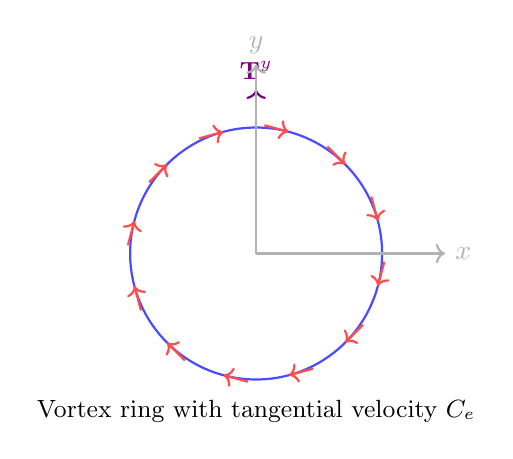
\begin{tikzpicture}[scale=0.8]
            % Ring (vortex core)
            \draw[thick, blue!70] (0,0) circle (2);

            % Flow lines (tangential swirl)
            \foreach \a in {15,45,75,105,135,165,195,225,255,285,315,345} {
                \draw[->, red!70, thick]
                ({2*cos(\a)}, {2*sin(\a)})
                ++({-0.4*sin(\a)}, {0.4*cos(\a)})
                -- ++({0.4*sin(\a)}, {-0.4*cos(\a)});
            }

            % Central torsion arrow
            \draw[->, thick, violet] (0,0) -- (0,2.6) node[above] {\small $\mathbf{T}^y$};

            % Axis labels
            \draw[->, thick, gray!60] (0,0) -- (3,0) node[right] {$x$};
            \draw[->, thick, gray!60] (0,0) -- (0,3) node[above] {$y$};

            % Label
            \node at (0,-2.5) {\small Vortex ring with tangential velocity $C_e$};
        \end{tikzpicture}
    \end{center}


    \noindent
    This diagram shows a vortex ring in the $x$-$y$ plane with tangential swirl velocity (red arrows) and central torsion aligned along the $y$-axis,
    representing $\mathbf{T}^y$ from Cartan's torsion 2-form.


    \section{Geometric Framework: Cartan's Structure Equations}\label{sec:framework}

Cartan's geometric formalism provides two fundamental structure equations on a manifold $\mathcal{M}$ equipped with coframe one-forms $\boldsymbol{\theta}^i$ and connection one-forms $\boldsymbol{\omega}^i{}_j$:
\begin{align}
    \text{Torsion 2-form:}\quad & \mathbf{T}^i = d\boldsymbol{\theta}^i + \boldsymbol{\omega}^i{}_j \wedge \boldsymbol{\theta}^j \\
    \text{Curvature 2-form:}\quad & \mathbf{R}^i{}_j = d\boldsymbol{\omega}^i{}_j + \boldsymbol{\omega}^i{}_k \wedge \boldsymbol{\omega}^k{}_j
\end{align}

In the Weitzenböck connection ($\boldsymbol{\omega}^i{}_j = 0$), all geometric deformation arises from torsion: $\mathbf{T}^i = d\boldsymbol{\theta}^i$, and $\mathbf{R}^i{}_j = 0$. Conversely, in the Levi-Civita connection (torsion-free), all deformation is encoded in curvature.

\section{Æther Interpretation in VAM}

In VAM, we associate:
\begin{itemize}
    \item $\boldsymbol{\theta}^i$: Local \ae ther displacement one-forms
    \item $\boldsymbol{\omega}^i{}_j$: Angular velocity of swirl (local rotational twist)
    \item $\mathbf{T}^i$: Core-induced torsion $\Rightarrow$ vortex dislocation (line defect)
    \item $\mathbf{R}^i{}_j$: Swirl curvature $\Rightarrow$ vortex disclination (rotational defect)
\end{itemize}

\section{Edge Dislocation in VAM as Torsion Source}

Consider a single vortex line (edge dislocation) along the $z$-axis with Burgers vector $\vec{b} = b\hat{x}$. The coframe is:
\begin{equation}
    \boldsymbol{\theta}^1 = dx + \frac{b}{2\pi} d\theta, \quad \boldsymbol{\theta}^2 = dy, \quad \boldsymbol{\theta}^3 = dz
\end{equation}

Using $d(d\theta) = 2\pi \delta(x)\delta(y) dx \wedge dy$, we compute:
\begin{align}
    \mathbf{T}^1 &= d\boldsymbol{\theta}^1 = b \delta(x) \delta(y) dx \wedge dy \\
    \mathbf{T}^2 &= 0, \quad \mathbf{T}^3 = 0
\end{align}

The dual vortex density becomes:
\begin{equation}
    \alpha^1 = *\mathbf{T}^1 = b \delta(x)\delta(y) \, dz
\end{equation}

\section{Equivalence to Wedge Disclination Dipole}

Following~\cite{kobayashi2025}, we reinterpret the same geometry using the Levi-Civita connection:
\begin{equation}
    \mathbf{R}^1{}_2 = \phi [\delta(x - L) - \delta(x + L)] \delta(y) dx \wedge dy
\end{equation}
where $\phi = b \rho$ encodes the Frank vector.

\begin{equation}
    \boxed{\text{Edge Dislocation} \equiv \text{Dipole of Wedge Disclinations}}
\end{equation}


    \section{Biot--Savart Swirl Integral in \ae ther}\label{sec:biot-savart}

Using the Biot--Savart analogy:
\begin{equation}
    \chi^i(\vec{x}) = \frac{1}{4\pi} \int \frac{\alpha^i(\vec{\xi}) \times (\vec{x} - \vec{\xi})}{|\vec{x} - \vec{\xi}|^3} \, d^3\xi
\end{equation}

The swirl potential $\chi^i$ defines the \ae theric coframe:
\begin{equation}
    \boldsymbol{\theta}^i = dx^i + \chi^i
\end{equation}

\section{Photon as a Vortex Ring}

The photon is modeled as a massless, quantized vortex ring with tangential velocity $C_e$ and core radius $r_c$, moving through the \ae ther. Its circulation is $\Gamma = 2\pi r_c C_e$.

\subsection{Lagrangian}
\begin{equation}
    \mathcal{L}_\gamma = \pi^2 r_c^2 C_e^2 \rho_\text{\ae}^{(\text{energy})} R_\gamma \left( \ln\left( \frac{8R_\gamma}{r_c} \right) - \frac{7}{4} \right)
\end{equation}

\subsection{Hamiltonian}
\begin{equation}
    \mathcal{H}_\gamma = \frac{P^2}{2M_{\text{ring}}} + \mathcal{L}_\gamma, \quad M_{\text{ring}} = \rho_\text{\ae}^{(\text{mass})} \cdot V_{\text{ring}}
\end{equation}

\subsection{Jacobian}
\begin{align}
    \vec{X}(\phi,\theta) =
    \begin{pmatrix}
    (R + a\cos\theta)\cos\phi \\
    (R + a\cos\theta)\sin\phi \\
    a\sin\theta
    \end{pmatrix}, \\
    J = a(R + a\cos\theta)
\end{align}


\section{Time Dilation and Proper Time in Photons}

Using swirl-induced time dilation~\cite{VAM-1}:
\begin{equation}
    \frac{dt}{dt_\infty} = \sqrt{1 - \frac{|\vec{\omega}|^2}{c^2}}, \quad \vec{\omega} = \frac{C_e}{r_c} \gg c \Rightarrow dt \approx 0
\end{equation}



    \section{Related Work and Historical Context}

The idea of a structured medium underpinning physical phenomena has deep historical roots. Lord Kelvin and Helmholtz first proposed vortex atom models~\cite{thomson1867}, attempting to derive material properties from knotted fluid structures. Maxwell~\cite{maxwell1861} and Lorentz~\cite{lorentz1904} further developed mechanical æther models to explain electromagnetism, before Einstein's relativity discouraged a privileged reference frame.

Contemporary approaches have revisited these ideas under new lights. In analogue gravity, Unruh~\cite{unruh1981} and Barceló et al.~\cite{barcelo2011} demonstrated that perturbations in a moving fluid obey effective relativistic wave equations, giving rise to phenomena like horizon analogs and Hawking radiation. Volovik~\cite{volovik2003} extended this to quantum fluids, proposing that all fields and metrics may arise from low-energy excitations in a condensed background.

In photonics, topological concepts have flourished. Lu et al.~\cite{lu2014} and Ozawa et al.~\cite{ozawa2019} showed that photonic crystals and metamaterials can simulate topological phases, suggesting deep connections between light, geometry, and protected vortex-like modes. These developments resonate strongly with the VAM perspective, where photons are topologically stable vortex excitations in a real fluid medium.

Unlike purely analogue models, VAM posits that the æther is not merely an emergent description but a physically real medium, with its own fundamental properties. In this sense, the model revives and modernizes early æther theories while remaining consistent with relativistic symmetry—much like how effective field theories respect renormalization group invariance without requiring spacetime fundamentalism.

\begin{quote}
    \emph{VAM bridges 19th-century æther mechanics with 21st-century topological and analogue models, offering a unified fluid-dynamical foundation for matter and radiation.}
\end{quote}


\section{Conclusion and Outlook}

    We have presented a unified interpretation of the photon as a topologically stable vortex ring within the Vortex \ae ther Model (VAM). Using Cartan’s structure equations, we mapped torsion and curvature to fundamental vortex phenomena: dislocations (vortex cores) and disclinations (swirl distortions), respectively. The photon emerges naturally in this geometric fluid framework as a quantized ring-like structure with null proper time, encapsulating both energy propagation and rotational æther dynamics.


    By deriving its Lagrangian, Hamiltonian, and Jacobian from first principles—selecting the appropriate form of æther density for each physical context—we confirmed the internal coherence of the model. The photon's behavior becomes a consequence of vortex stability, quantized circulation, and localized energy-momentum flow in the æther.


    This approach offers several exciting implications:

    \begin{itemize}

    \item It provides a hydrodynamic foundation for gauge bosons, potentially extendable to W, Z, and gluons as knotted or linked vortex structures.

    \item The link between torsion and electrodynamics may enable a geometric unification of Maxwell’s equations with the topology of flow defects.

    \item VAM’s reinterpretation of light as fluid rotation suggests experimental pathways using superfluid analogs to probe photon structure, birefringence, or vacuum dispersion.

    \end{itemize}


    Future work will focus on generalizing this vortex-ring construction to incorporate spin-1/2 particles as twisted torus knots, analyzing photon-photon scattering via knot interactions, and embedding this framework into the topological fluid reinterpretation of the Standard Model.


    \medskip

    \noindent\textbf{Key Prediction:} The photon's zero-rest-mass arises not from symmetry breaking, but from a topological constraint enforcing null ætheric proper time: a perpetual rotation with velocity $C_e$ yields $ds^2 = 0$.


    \medskip

    \noindent This framework suggests a radical rethinking of particle ontology: not as pointlike fields in curved spacetime, but as structured flows in a flat, rotating æther.

    \appendix
    \section{Lagrangian, Hamiltonian, and Jacobian Formulation of a Vortex Ring in the Vortex \AE ther Model (VAM)}

    \subsection{Jacobian for a Vortex Ring Flow Field}
    Consider a vortex ring with core radius $r_c$, circulation $\Gamma$, and cylindrical symmetry. The velocity field $\vec{v}(\vec{x})$ of such a vortex in cylindrical coordinates $(r, \phi, z)$ can be modeled with azimuthal symmetry:
    \begin{equation}
        \vec{v}(r, z) = v_r(r, z)\hat{r} + v_z(r, z)\hat{z}
    \end{equation}
    with vorticity only in the $\phi$-direction: $\vec{\omega} = \omega_\phi(r, z)\hat{\phi}$.

    The Jacobian matrix of the flow $\vec{v}(\vec{x})$ is defined as:
    \begin{equation}
        J_{ij} = \frac{\partial v_i}{\partial x_j}
    \end{equation}
    This is used to compute the vorticity and strain-rate tensor. For incompressible flow $\div \vec{v} = 0$, so $\mathrm{Tr}(J) = 0$. The antisymmetric part yields:
    \begin{equation}
        \omega_i = \epsilon_{ijk} \partial_j v_k = (\nabla \times \vec{v})_i
    \end{equation}

    \subsection{Lagrangian Density of a Vortex Ring in VAM}
    From \cite{VAM-1,VAM-2,VAM-0}, the VAM Lagrangian is constructed from the kinetic swirl energy and vortex helicity. We define:
    \begin{equation}
        \mathcal{L} = \frac{1}{2} \rho_\text{\ae}^{(\text{fluid})} \vec{v}^{2} - \lambda \vec{v} \cdot (\nabla \times \vec{v})
    \end{equation}
    where $\lambda$ is a coupling constant with dimensions $[\text{time} \cdot \text{length}^2]$. In VAM, helicity represents charge-like conservation:\cite{VAM-5,VAM-6}

    Let us consider the ring with azimuthal velocity $v_\phi = \frac{\Gamma}{2\pi r}$ localized within the vortex core of radius $r_c$, and assume uniform vorticity inside:
    \begin{equation}
        \vec{\omega} = \nabla \times \vec{v} = \omega_0\hat{\phi}, \qquad \omega_0 = \frac{\Gamma}{\pi r_c^2}
    \end{equation}
    The energy per unit length is then:
    \begin{equation}
        \mathcal{E} = \int_0^{r_c} \left[ \frac{1}{2} \rho_\text{\ae}^{(\text{fluid})} \left( \frac{\Gamma}{2\pi r} \right)^2 - \lambda \frac{\Gamma}{2\pi r} \cdot \omega_0 \right] 2\pi r \, dr
    \end{equation}

    Evaluating the integral yields the effective Lagrangian per unit length of the ring:
    \begin{equation}
        \mathcal{L}_\text{ring} = \frac{\rho_\text{\ae}^{(\text{fluid})} \Gamma^2}{4\pi} \ln\left( \frac{r_c}{\delta} \right) - \lambda \Gamma \omega_0 r_c^2
    \end{equation}
    where $\delta$ is a vortex core cutoff.

    \subsection{Hamiltonian of a Vortex Ring in VAM}
    The canonical momentum density is:
    \begin{equation}
        \vec{\pi} = \pdv{\mathcal{L}}{\vec{v}} = \rho_\text{\ae}^{(\text{fluid})} \vec{v} - \lambda \vec{\omega}
    \end{equation}
    Then the Hamiltonian density is:
    \begin{equation}
        \mathcal{H} = \vec{\pi} \cdot \vec{v} - \mathcal{L} = \frac{1}{2} \rho_\text{\ae}^{(\text{fluid})} \vec{v}^2 + \lambda \vec{v} \cdot \vec{\omega}
    \end{equation}

    For the vortex ring, inserting the same field approximations as before:
    \begin{equation}
        \mathcal{H}_\text{ring} = \int_0^{r_c} \left[ \frac{1}{2} \rho_\text{\ae}^{(\text{fluid})} \left( \frac{\Gamma}{2\pi r} \right)^2 + \lambda \frac{\Gamma}{2\pi r} \cdot \omega_0 \right] 2\pi r \, dr
    \end{equation}

    Which yields:
    \begin{equation}
        \mathcal{H}_\text{ring} = \frac{\rho_\text{\ae}^{(\text{fluid})} \Gamma^2}{4\pi} \ln\left( \frac{r_c}{\delta} \right) + \lambda \Gamma \omega_0 r_c^2
    \end{equation}

    \subsection{Conclusion}
    The Jacobian characterizes the local deformation due to flow. The Lagrangian encodes energy and helicity structure of the vortex. The Hamiltonian recovers total energetic contribution of the vortex ring. In the VAM framework, this triad provides a fully vorticity-based alternative to point-particle or field-theoretic formulations.
% ============= END of content ============

    \bibliographystyle{unsrt}
    \bibliography{photon_vortex_refs}

\end{document}